\documentclass[11pt,english]{article}
%\usepackage{times}
\usepackage[T1]{fontenc}
\usepackage[authoryear]{natbib}
\usepackage{amssymb,amsmath,amsthm}
%\usepackage[nolists]{endfloat}
\usepackage{graphicx}
\usepackage{chngpage}
\usepackage[hang, small]{caption} % Custom captions under/above floats in tables or figures
\usepackage{pdflscape}
\usepackage{longtable}
\usepackage{color}
\usepackage{epigraph}
\usepackage{float}
\usepackage{array}
\usepackage{fullpage}
\usepackage{setspace}
\usepackage[normalem]{ulem}
\usepackage{appendix}
\usepackage{booktabs}
\usepackage{multirow}
\usepackage[small,compact]{titlesec}
\usepackage{rotate}
\usepackage{subcaption}
\usepackage{titletoc}
\usepackage{threeparttable}
\usepackage[pdfborder={0 0 0}]{hyperref}


\newtheorem{definition}{Definition}
\newtheorem{hypothesis}{Hypothesis}
\newtheorem{lemma}{Lemma}
\newtheorem{corollary}{Corollary}
\newtheorem{theorem}{Theorem}

\setlength{\epigraphwidth}{.5\textwidth}


\newcommand{\note}[1]{
  {\color{red} #1 }
}

\begin{document}

\title{Modern Man Challenge: Preliminary Results}

\author{
  Jeannie Annan\footnote{International Rescue Committee and University of Chicago, \href{Jeannie.Annan@rescue.org}{Jeannie.Annan@rescue.org}} \quad  
  Gunther Fink\footnote{Swiss Tropical and Public Health Institute, \href{guenther.fink@swisstph.ch }{guenther.fink@swisstph.ch }} \quad  
  Betsy Levy Paluck\footnote{Princeton University, \href{epaluck@princeton.edu}{epaluck@princeton.edu}}\thanks{
  [THANKS]
  } 
}


\maketitle

%\textbf{Keywords}: ***

%\begin{abstract}
%  ABSTRACT
%\end{abstract}


\clearpage

\tableofcontents

\newpage

\listoftables

\newpage

\setcounter{page}{1}

\doublespacing 

\section{Intent-to-Treat Effects}

\subsection{Regression specifications}

Pre-liminary results are estimated using two different regressions specifications. The unadjusted estimator is a least squares regression that conditions on an indicator for the treatment assignment $Z_i$ with standard errors estimated using the wild-cluster bootstrap to account for the small number of clusters ($N = 16$), i.e.:

\[Y_{ij} = \beta_0 + \beta_1 Z_i + \varepsilon_i \]

The adjusted estimator additionally conditions on a vector of mean-centered covariates, $\overline{X}_i$, comprising:
\begin{itemize}
\item baseline measures assessed during a household survey in 2018.
\item endline measures assumed to be time invariant assessed in 2019.
\item retrospective reports of pre-treatment violence asssessed in 2019 but referring to the 5 months prior to Christmas 2018.
\end{itemize} 
For each outcome the set of covariates in $\overline{X}_i$ are selected via the lasso. The adjusted estimator also includes covariate by treatment interaction terms as suggested in Lin (2013):
\[Y_{ij} = \beta_0 + \beta_1 Z_i + \beta_2 \overline{X}_i + \beta_3 Z_i \overline{X}_i + \varepsilon_i\]

In both specifications $\beta_1$ estimates the intention-to-treat effect of the Modern Man Challenge. 

\subsection{Primary Outcomes}

\subsubsection{IPV}

\begin{table}[H]
\centering

\begin{tabular}{l c c c c c c}
\toprule
 & IPV & IPV & Physical/Sexual & Physical/Sexual & Emotional & Emotional \\
\midrule
MMC                 & $0.142$        & $0.133$       & $0.111$        & $0.106$       & $0.110$        & $0.066$       \\
                    & $(0.085)$      & $(0.156)$     & $(0.141)$      & $(0.133)$     & $(0.059)$      & $(0.125)$     \\
Constant            & $-0.083$       & $-0.078$      & $-0.086$       & $-0.066$      & $-0.037$       & $-0.034$      \\
                    & $(0.064)$      & $(0.074)$     & $(0.063)$      & $(0.081)$     & $(0.054)$      & $(0.067)$     \\
\midrule
Bootstrap $p$-value & $0.123$        & $0.422$       & $0.406$        & $0.456$       & $0.086$        & $0.631$       \\
Covariates          & $\textrm{Yes}$ & $\textrm{No}$ & $\textrm{Yes}$ & $\textrm{No}$ & $\textrm{Yes}$ & $\textrm{No}$ \\
Clusters            & $16$           & $16$          & $16$           & $16$          & $16$           & $16$          \\
Observations        & $455$          & $455$         & $455$          & $455$         & $455$          & $455$         \\
Adj. R$^2$          & $0.422$        & $0.003$       & $0.386$        & $0.002$       & $0.416$        & $-0.001$      \\
\bottomrule
\multicolumn{7}{l}{\scriptsize{\parbox{\linewidth}{\vspace{2pt} 
       \textit{Notes:} Estimates of the intent-to-treat effects of Modern Man mobile 
       messaging program on pre-registered primary outcomes using adjusted regression 
       specification based on the Lin 2013 estimator with CR2 cluster-robust 
       standard errors in parentheses. Columns 1 and 2 are a composite index of 
       acts of intimate partner violence. Columns 3 and 4 are a composite index of acts
       of physical violence. Columns 5 and 6 are a composite index of acts of sexual violence.
       All indices were constructed using the first factor from IRT models of subitems. 
       Bootstrap $p$-value estimated using 10,000 replicates of wild cluster bootstrap-$t$. \\ $^{***}p<0.001$; $^{**}p<0.01$; $^{*}p<0.05$.}}}
\end{tabular}

\caption{ITT effects on indices of intimate partner violence since Christmas 2018.}
\label{tab:ipv}
\end{table}

\begin{figure}[H]
\centering
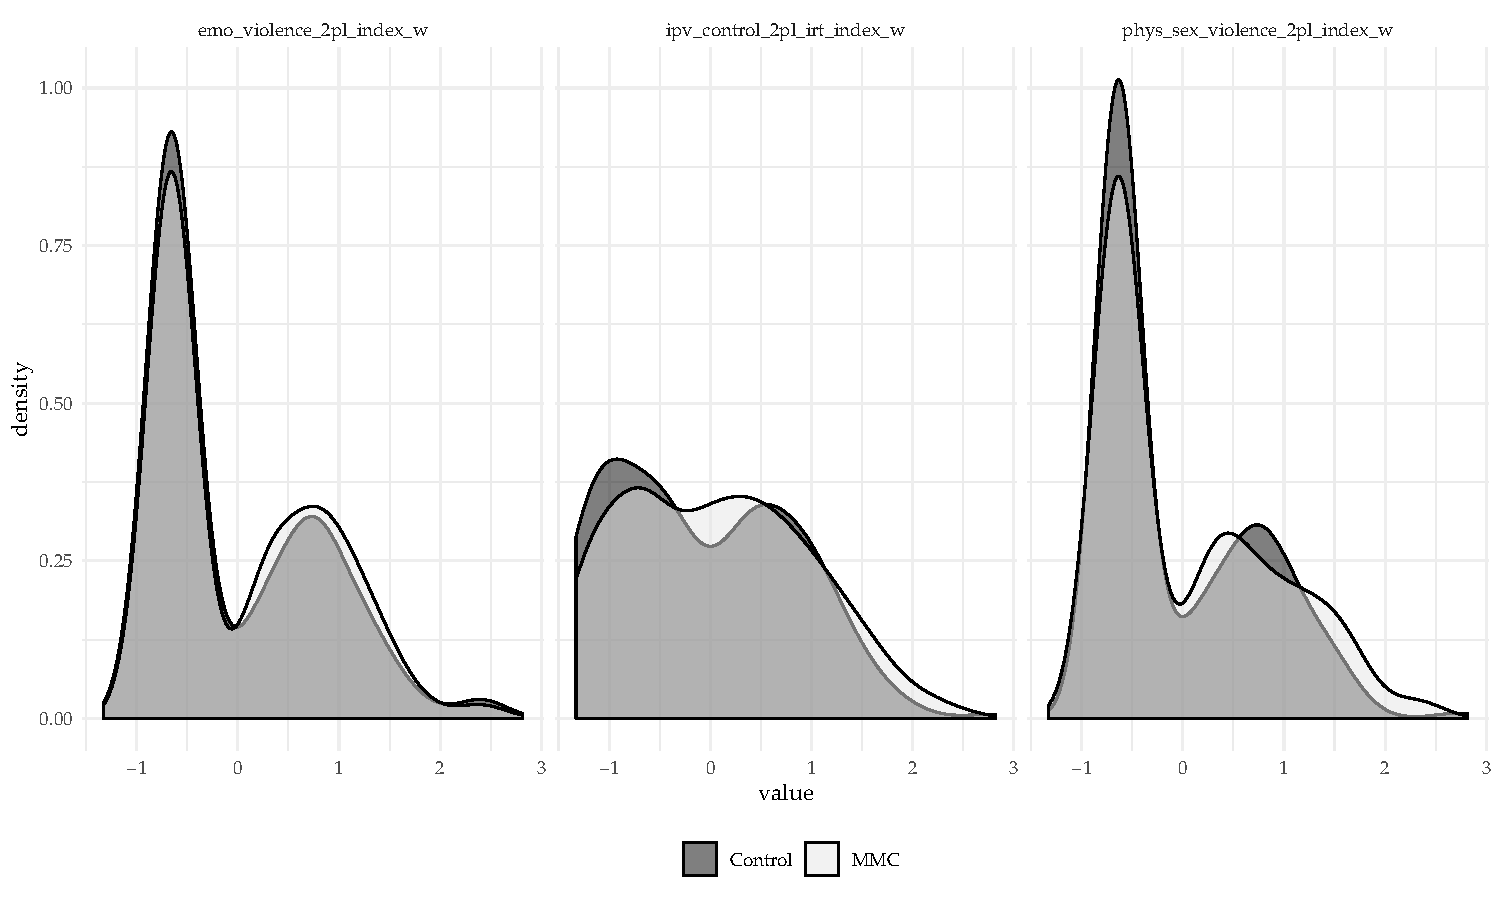
\includegraphics[width = \textwidth]{figures/densities.pdf}
\caption{Comparison of densities of violence indices by treatment status.}
\label{fig:densities}
\end{figure}

\subsubsection{Subitems}

\begin{figure}[H]
\centering
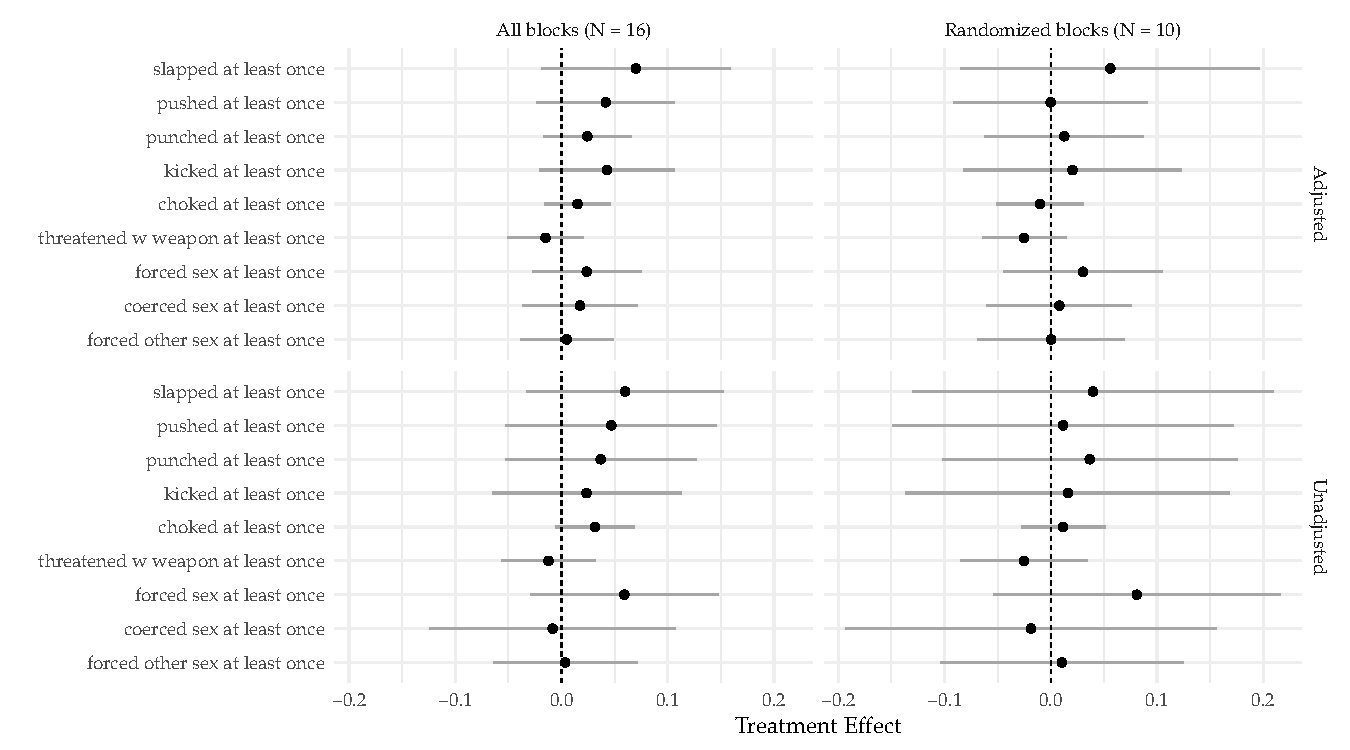
\includegraphics[width = \textwidth]{figures/subitem_plot.pdf}
\caption{Plot of ITT effects on index subitems for violence outcomes.}
\label{fig:subitem_plot}
\end{figure}

\subsection{Men's Secondary Outcomes}

\subsubsection{Attitudes and perceptions about violence}

\begin{table}[H]
\centering

\begin{tabular}{l c c c c}
\toprule
 & Justifies Violence & Justifies Violence & \shortstack{Perceptions of \\ Violence Norms} & \shortstack{Perceptions of \\ Violence Norms} \\
\midrule
MMC                 & $-0.008$       & $-0.034$      & $0.257$        & $0.224$        \\
                    & $(0.110)$      & $(0.116)$     & $(0.248)$      & $(0.304)$      \\
Constant            & $0.356^{***}$  & $0.361^{***}$ & $-3.191^{***}$ & $-3.174^{***}$ \\
                    & $(0.076)$      & $(0.080)$     & $(0.085)$      & $(0.124)$      \\
\midrule
Bootstrap $p$-value & $0.944$        & $0.762$       & $0.344$        & $0.482$        \\
Covariates          & $\textrm{Yes}$ & $\textrm{No}$ & $\textrm{Yes}$ & $\textrm{No}$  \\
Clusters            & $16$           & $16$          & $16$           & $16$           \\
Observations        & $455$          & $455$         & $455$          & $455$          \\
Adj. R$^2$          & $0.022$        & $-0.002$      & $0.040$        & $0.000$        \\
\bottomrule
\multicolumn{5}{l}{\scriptsize{\parbox{\linewidth}{\vspace{2pt}
       \textit{Notes:} Estimates of the intent-to-treat effects of Modern Man mobile
       messaging program on secondary men's outcomes using adjusted regression
       specification based on the Lin 2013 estimator with CR2 cluster-robust
       standard errors in parentheses. Columns 1 and 2 are a composite index of
       whether man's attitudes justify use of violence against women. Columns 3 and 4
       are a composite index of men's perceptions about whether their community justifies
       the use of violence. All indices were constructed as sums of subitems coded in
       same substantive direction. Bootstrap $p$-value estimated using 10,000 replicates of 
       wild cluster bootstrap-$t$. \\ $^{***}p<0.001$; $^{**}p<0.01$; $^{*}p<0.05$.}}}
\end{tabular}

\caption{ITT effects on on indices of men's attitudes and perceptions of violence since Christmas 2018.}
\label{tab:attitudes_results_m}
\end{table}

\subsubsection{Decision-making}

\begin{table}[H]
\centering

\begin{tabular}{l c c c c}
\toprule
 & Decision-making & Decision-making & Man feels supported & Man feels supported \\
\midrule
MMC                 & $0.823^{**}$   & $0.725^{*}$   & $0.205$        & $-0.005$      \\
                    & $(0.311)$      & $(0.366)$     & $(0.243)$      & $(0.290)$     \\
Constant            & $7.046^{***}$  & $7.114^{***}$ & $8.195^{***}$  & $8.311^{***}$ \\
                    & $(0.262)$      & $(0.327)$     & $(0.182)$      & $(0.148)$     \\
\midrule
Bootstrap $p$-value & $0.025$        & $0.088$       & $0.402$        & $0.986$       \\
Covariates          & $\textrm{Yes}$ & $\textrm{No}$ & $\textrm{Yes}$ & $\textrm{No}$ \\
Clusters            & $16$           & $16$          & $16$           & $16$          \\
Observations        & $455$          & $455$         & $455$          & $455$         \\
Adj. R$^2$          & $0.146$        & $0.023$       & $0.083$        & $-0.002$      \\
\bottomrule
\multicolumn{5}{l}{\scriptsize{\parbox{\linewidth}{\vspace{2pt}
       \textit{Notes:} Estimates of the intent-to-treat effects of Modern Man mobile
       messaging program on secondary men's outcomes using adjusted regression
       specification based on the Lin 2013 estimator with CR2 cluster-robust
       standard errors in parentheses. Columns 1 and 2 are a composite index of
       women's involvement in decision-making. Columns 3 and 4 are a composite index of 
       whether men feel supported by their partner. All indices were constructed as sums of 
       subitems coded in same substantive direction. Bootstrap $p$-value estimated using 10,000
       replicates of wild cluster bootstrap-$t$. \\ $^{***}p<0.001$; $^{**}p<0.01$; $^{*}p<0.05$.}}}
\end{tabular}

\caption{ITT effects on on indices of men's reports of decision-making and support since Christmas 2018.}
\label{tab:dm_etc_results_m}
\end{table}

\subsubsection{Sexual consent and pleasure}

\begin{table}[H]
\centering

\begin{tabular}{l c c c c}
\toprule
 & \shortstack{Neg. response \\ to no consent} & \shortstack{Neg. response \\ to no consent} & Values woman's pleasure & Values woman's pleasure \\
\midrule
MMC                 & $-0.071$       & $-0.074$      & $0.438^{**}$   & $0.429^{*}$   \\
                    & $(0.053)$      & $(0.055)$     & $(0.149)$      & $(0.190)$     \\
Constant            & $1.026^{***}$  & $1.027^{***}$ & $5.096^{***}$  & $5.100^{***}$ \\
                    & $(0.036)$      & $(0.037)$     & $(0.099)$      & $(0.115)$     \\
\midrule
Bootstrap $p$-value & $0.194$        & $0.199$       & $0.014$        & $0.037$       \\
Covariates          & $\textrm{Yes}$ & $\textrm{No}$ & $\textrm{Yes}$ & $\textrm{No}$ \\
Clusters            & $16$           & $16$          & $16$           & $16$          \\
Observations        & $455$          & $455$         & $455$          & $455$         \\
Adj. R$^2$          & $0.012$        & $0.001$       & $0.023$        & $0.002$       \\
\bottomrule
\multicolumn{5}{l}{\scriptsize{\parbox{\linewidth}{\vspace{2pt}
       \textit{Notes:} Estimates of the intent-to-treat effects of Modern Man mobile
       messaging program on secondary men's outcomes using adjusted regression
       specification based on the Lin 2013 estimator with CR2 cluster-robust
       standard errors in parentheses. Columns 1 and 2 are a composite index of
       whether the man justifies negative responses to woman's refusal of sex. Columns 3 and 4
       are a composite index of men's value of woman's pleasure during sex. All indices were
       constructed as sums of subitems coded insame substantive direction. 
       Bootstrap $p$-value estimated using 10,000 replicates of wild cluster bootstrap-$t$. \\ $^{***}p<0.001$; $^{**}p<0.01$; $^{*}p<0.05$.}}}
\end{tabular}

\caption{ITT effects on on indices of men's reports of sexual consent practices and pleasure since Christmas 2018.}
\label{tab:sex_results_m}
\end{table}

\subsubsection{Communication}

\begin{table}[H]
\centering

\begin{tabular}{l c c c c c c c c}
\toprule
 & \shortstack{Discuss \\ relation- \\ ship} & \shortstack{Discuss \\ relation- \\ ship} & \shortstack{Good \\ talk} & \shortstack{Good \\ talk} & \shortstack{Freq. \\ good \\ expressions} & \shortstack{Freq. \\ good \\ expressions} & \shortstack{Enjoy \\ mutual \\ acts} & \shortstack{Enjoy \\ mutual \\ acts} \\
\midrule
MMC                 & $0.292$        & $0.349$        & $0.115$        & $0.115$        & $0.511$        & $0.323$        & $0.957$        & $0.625$        \\
                    & $(0.255)$      & $(0.258)$      & $(0.225)$      & $(0.225)$      & $(0.575)$      & $(0.642)$      & $(0.979)$      & $(0.892)$      \\
Constant            & $11.742^{***}$ & $11.799^{***}$ & $11.516^{***}$ & $11.516^{***}$ & $30.365^{***}$ & $30.511^{***}$ & $35.717^{***}$ & $36.205^{***}$ \\
                    & $(0.207)$      & $(0.225)$      & $(0.177)$      & $(0.177)$      & $(0.328)$      & $(0.414)$      & $(0.817)$      & $(0.708)$      \\
\midrule
Bootstrap $p$-value & $0.292$        & $0.224$        & $0.628$        & $0.628$        & $0.373$        & $0.604$        & $0.358$        & $0.505$        \\
Covariates          & $\textrm{Yes}$ & $\textrm{No}$  & $\textrm{Yes}$ & $\textrm{No}$  & $\textrm{Yes}$ & $\textrm{No}$  & $\textrm{Yes}$ & $\textrm{No}$  \\
Clusters            & $16$           & $16$           & $16$           & $16$           & $16$           & $16$           & $16$           & $16$           \\
Observations        & $455$          & $455$          & $455$          & $455$          & $455$          & $455$          & $455$          & $455$          \\
Adj. R$^2$          & $0.045$        & $0.002$        & $-0.002$       & $-0.002$       & $0.028$        & $-0.002$       & $0.041$        & $-0.000$       \\
\bottomrule
\multicolumn{9}{l}{\scriptsize{\parbox{\linewidth}{\vspace{2pt}
       \textit{Notes:} Estimates of the intent-to-treat effects of Modern Man mobile
       messaging program on secondary men's outcomes using adjusted regression
       specification based on the Lin 2013 estimator with CR2 cluster-robust
       standard errors in parentheses. Columns 1 and 2 are a composite index of
       how often the couple discusses relationship and household practicalities. 
       Columns 3 and 4 are a composite index of couple's shared discussion about each other.
       Columns 5 and 6 are a composite index of frequency of good expressions between couple.
       Columns 7 and 8 are a composite index of the man's enjoyment of mutual activities with 
       his female partner. All indices were constructed as sums of subitems coded in
       same substantive direction. Bootstrap $p$-value estimated using 10,000 replicates of wild
       cluster bootstrap-$t$. \\ $^{***}p<0.001$; $^{**}p<0.01$; $^{*}p<0.05$.}}}
\end{tabular}

\caption{ITT effects on on indices of men's reports of communication practices since Christmas 2018.}
\label{tab:comm_results_m}
\end{table}

\subsubsection{Conflict}

\begin{table}[H]
\centering

\begin{tabular}{l c c c c c c c c}
\toprule
 & \shortstack{Resolve \\ conflicts} & \shortstack{Resolve \\ conflicts} & \shortstack{Freq. \\ argue} & \shortstack{Freq. \\ argue} & \shortstack{Woman's \\ resolution \\ skills} & \shortstack{Woman's \\ resolution \\ skills} & \shortstack{Man's \\ emotional \\ reg.} & \shortstack{Man's \\ emotional \\ reg.} \\
\midrule
MMC          & $-0.086$       & $-0.086$      & $-0.318$       & $-0.486$      & $0.250$        & $0.190$        & $1.140^{*}$    & $0.799$        \\
             & $(0.134)$      & $(0.135)$     & $(0.487)$      & $(0.523)$     & $(0.261)$      & $(0.266)$      & $(0.548)$      & $(0.537)$      \\
Constant     & $1.525^{***}$  & $1.525^{***}$ & $8.074^{***}$  & $8.186^{***}$ & $10.752^{***}$ & $10.764^{***}$ & $16.739^{***}$ & $16.914^{***}$ \\
             & $(0.074)$      & $(0.075)$     & $(0.241)$      & $(0.363)$     & $(0.184)$      & $(0.195)$      & $(0.397)$      & $(0.448)$      \\
\midrule
Covariates   & $\textrm{Yes}$ & $\textrm{No}$ & $\textrm{Yes}$ & $\textrm{No}$ & $\textrm{Yes}$ & $\textrm{No}$  & $\textrm{Yes}$ & $\textrm{No}$  \\
Clusters     & $16$           & $16$          & $16$           & $16$          & $16$           & $16$           & $16$           & $16$           \\
Observations & $583$          & $583$         & $583$          & $583$         & $583$          & $583$          & $583$          & $583$          \\
Adj. R$^2$   & $-0.001$       & $-0.001$      & $0.156$        & $0.001$       & $0.019$        & $-0.001$       & $0.106$        & $0.002$        \\
\bottomrule
\multicolumn{9}{l}{\scriptsize{\parbox{\linewidth}{\vspace{2pt}
       \textit{Notes:} Estimates of the intent-to-treat effects of Modern Man mobile
       messaging program on secondary men's outcomes using adjusted regression
       specification based on the Lin 2013 estimator with wild cluster bootstrap
       standard errors in parentheses. Columns 1 and 2 are a composite index of
       the man's report of the couple's ability to resolve conflict. Columns 3 and 4
       are a composite index of the man's report of how frequently he and his partner argue. 
       Columns 5 and 6 are a composite index of the man's report of his partner's positive conflict 
       resolution skills. Columns 7 and 8 are a composite index of the man's ability to emotionally regulate
       during conflict. All indices were constructed as sums of subitems coded in same 
       substantive direction. Bootstrapped standard errors estimated using 10,000 replicates. \\ $^{***}p<0.001$; $^{**}p<0.01$; $^{*}p<0.05$.}}}
\end{tabular}

\caption{ITT effects on on indices of men's reports of conflict since Christmas 2018.}
\label{tab:conflict_results_m}
\end{table}

\subsection{Women's Secondary Outcomes}


\subsubsection{Attitudes and perceptions about violence}

\begin{table}[H]
\centering

\begin{tabular}{l c c c c}
\toprule
 & Justifies Violence & Justifies Violence & Perceptions of Violence & Perceptions of Violence \\
\midrule
MMC          & $-0.240$       & $-0.252^{*}$  & $-0.775^{*}$   & $-0.829^{*}$   \\
             & $(0.128)$      & $(0.128)$     & $(0.309)$      & $(0.353)$      \\
Constant     & $1.012^{***}$  & $1.018^{***}$ & $-1.535^{***}$ & $-1.511^{***}$ \\
             & $(0.082)$      & $(0.083)$     & $(0.263)$      & $(0.311)$      \\
\midrule
Covariates   & $\textrm{Yes}$ & $\textrm{No}$ & $\textrm{Yes}$ & $\textrm{No}$  \\
Clusters     & $16$           & $16$          & $16$           & $16$           \\
Observations & $583$          & $583$         & $583$          & $583$          \\
Adj. R$^2$   & $0.013$        & $0.007$       & $0.053$        & $0.014$        \\
\bottomrule
\multicolumn{5}{l}{\scriptsize{\parbox{\linewidth}{\vspace{2pt}
       \textit{Notes:} Estimates of the intent-to-treat effects of Modern Man mobile
       messaging program on secondary women's outcomes using adjusted regression
       specification based on the Lin 2013 estimator with wild cluster bootstrap
       standard errors in parentheses. Columns 1 and 2 are a composite index of
       whether woman's attitudes justify use of violence against women. Columns 3 and 4
       are a composite index of women's perceptions about whether their community justifies
       the use of violence. All indices were constructed as sums of subitems coded in
       same substantive direction. Bootstrapped standard errors estimated using 10,000 replicates. \\ $^{***}p<0.001$; $^{**}p<0.01$; $^{*}p<0.05$.}}}
\end{tabular}

\caption{ITT effects on on indices of women's attitudes and perceptions of violence since Christmas 2018.}
\label{tab:attitudes_results_w}
\end{table}

\subsubsection{Decision-making}

\begin{table}[H]
\centering

\begin{tabular}{l c c c c}
\toprule
 & Decision-making & Decision-making & Woman feels supported & Woman feels supported \\
\midrule
MMC                 & $-0.345^{*}$   & $-0.357^{*}$  & $-0.271$       & $-0.326$      \\
                    & $(0.161)$      & $(0.167)$     & $(0.280)$      & $(0.352)$     \\
Constant            & $7.524^{***}$  & $7.548^{***}$ & $7.347^{***}$  & $7.352^{***}$ \\
                    & $(0.098)$      & $(0.121)$     & $(0.131)$      & $(0.175)$     \\
\midrule
Bootstrap $p$-value & $0.043$        & $0.040$       & $0.326$        & $0.364$       \\
Covariates          & $\textrm{Yes}$ & $\textrm{No}$ & $\textrm{Yes}$ & $\textrm{No}$ \\
Clusters            & $16$           & $16$          & $16$           & $16$          \\
Observations        & $455$          & $455$         & $455$          & $455$         \\
Adj. R$^2$          & $0.043$        & $0.005$       & $0.025$        & $0.002$       \\
\bottomrule
\multicolumn{5}{l}{\scriptsize{\parbox{\linewidth}{\vspace{2pt}
       \textit{Notes:} Estimates of the intent-to-treat effects of Modern Man mobile
       messaging program on secondary women's outcomes using adjusted regression
       specification based on the Lin 2013 estimator with CR2 cluster-robust
       standard errors in parentheses. Columns 1 and 2 are a composite index of
       women's involvement in decision-making. Columns 3 and 4 are a composite index of 
       whether women feel supported by their partner. All indices were constructed as sums of 
       subitems coded in same substantive direction. Bootstrap $p$-value estimated using 10,000 replicates of wild cluster bootstrap-$t$. \\ $^{***}p<0.001$; $^{**}p<0.01$; $^{*}p<0.05$.}}}
\end{tabular}

\caption{ITT effects on on indices of women's reports of decision-making and support since Christmas 2018.}
\label{tab:dm_etc_results_w}
\end{table}

\subsubsection{Sexual consent and pleasure}

\begin{table}[H]
\centering

\begin{tabular}{l c c}
\toprule
 & \shortstack{Neg. response \\ to no consent} & \shortstack{Neg. response \\ to no consent} \\
\midrule
MMC          & $-0.052$       & $-0.052$      \\
             & $(0.043)$      & $(0.043)$     \\
Constant     & $1.082^{***}$  & $1.082^{***}$ \\
             & $(0.034)$      & $(0.034)$     \\
\midrule
Covariates   & $\textrm{Yes}$ & $\textrm{No}$ \\
Clusters     & $16$           & $16$          \\
Observations & $583$          & $583$         \\
Adj. R$^2$   & $0.000$        & $0.000$       \\
\bottomrule
\multicolumn{3}{l}{\scriptsize{\parbox{\linewidth}{\vspace{2pt}
       \textit{Notes:} Estimates of the intent-to-treat effects of Modern Man mobile
       messaging program on secondary women's outcomes using adjusted regression
       specification based on the Lin 2013 estimator with wild cluster bootstrap
       standard errors in parentheses. Columns 1 and 2 are a composite index of
       whether the woman justifies negative responses to woman's refusal of sex. All indices were
       constructed as sums of subitems coded insame substantive direction. 
       Bootstrapped standard errors estimated using 10,000 replicates. \\ $^{***}p<0.001$; $^{**}p<0.01$; $^{*}p<0.05$.}}}
\end{tabular}

\caption{ITT effects on on indices of women's reports of sexual consent practices and pleasure since Christmas 2018.}
\label{tab:sex_results_w}
\end{table}

\subsubsection{Communication}

\begin{table}[H]
\centering

\begin{tabular}{l c c c c c c c c}
\toprule
 & Discuss relationship & Discuss relationship & Good talk & Good talk & Freq. good expressions & Freq. good expressions & Enjoy mutual acts & Enjoy mutual acts \\
\midrule
MMC          & $-0.139$       & $-0.198$       & $0.380$        & $0.319$       & $-0.344$       & $-0.465$       & $0.000$        & $-0.302$       \\
             & $(0.287)$      & $(0.304)$      & $(0.506)$      & $(0.537)$     & $(0.609)$      & $(0.653)$      & $(0.646)$      & $(0.824)$      \\
Constant     & $10.538^{***}$ & $10.561^{***}$ & $9.962^{***}$  & $9.968^{***}$ & $27.936^{***}$ & $27.993^{***}$ & $32.309^{***}$ & $32.500^{***}$ \\
             & $(0.163)$      & $(0.169)$      & $(0.361)$      & $(0.391)$     & $(0.392)$      & $(0.412)$      & $(0.338)$      & $(0.460)$      \\
\midrule
Covariates   & $\textrm{Yes}$ & $\textrm{No}$  & $\textrm{Yes}$ & $\textrm{No}$ & $\textrm{Yes}$ & $\textrm{No}$  & $\textrm{Yes}$ & $\textrm{No}$  \\
Clusters     & $16$           & $16$           & $16$           & $16$          & $16$           & $16$           & $16$           & $16$           \\
Observations & $583$          & $583$          & $583$          & $583$         & $583$          & $583$          & $583$          & $583$          \\
Adj. R$^2$   & $0.007$        & $-0.001$       & $0.016$        & $-0.000$      & $0.016$        & $-0.001$       & $0.066$        & $-0.001$       \\
\bottomrule
\multicolumn{9}{l}{\scriptsize{\parbox{\linewidth}{\vspace{2pt}
       \textit{Notes:} Estimates of the intent-to-treat effects of Modern Man mobile
       messaging program on secondary women's outcomes using adjusted regression
       specification based on the Lin 2013 estimator with wild cluster bootstrap
       standard errors in parentheses. Columns 1 and 2 are a composite index of
       how often the couple discusses relationship and household practicalities. 
       Columns 3 and 4 are a composite index of couple's shared discussion about each other.
       Columns 5 and 6 are a composite index of frequency of good expressions between couple.
       Columns 7 and 8 are a composite index of the woman's enjoyment of mutual activities with 
       her male partner. All indices were constructed as sums of subitems coded in
       same substantive direction. Bootstrapped standard errors estimated using 10,000 
       replicates. \\ $^{***}p<0.001$; $^{**}p<0.01$; $^{*}p<0.05$.}}}
\end{tabular}

\caption{ITT effects on on indices of women's reports of communication practices since Christmas 2018.}
\label{tab:comm_results_w}
\end{table}

\subsubsection{Conflict}

\begin{table}[H]
\centering

\begin{tabular}{l c c c c c c}
\toprule
 & \shortstack{Resolve \\ conflicts} & \shortstack{Resolve \\ conflicts} & \shortstack{Freq. argue} & \shortstack{Freq. argue} & \shortstack{Man's resolution \\ skills} & \shortstack{Man's resolution \\ skills} \\
\midrule
MMC          & $-0.074$       & $-0.079$      & $-0.295$       & $-0.249$      & $0.683$        & $0.626$        \\
             & $(0.093)$      & $(0.092)$     & $(0.385)$      & $(0.514)$     & $(0.398)$      & $(0.396)$      \\
Constant     & $1.298^{***}$  & $1.304^{***}$ & $9.360^{***}$  & $9.329^{***}$ & $10.077^{***}$ & $10.100^{***}$ \\
             & $(0.049)$      & $(0.049)$     & $(0.234)$      & $(0.274)$     & $(0.290)$      & $(0.291)$      \\
\midrule
Covariates   & $\textrm{Yes}$ & $\textrm{No}$ & $\textrm{Yes}$ & $\textrm{No}$ & $\textrm{Yes}$ & $\textrm{No}$  \\
Clusters     & $16$           & $16$          & $16$           & $16$          & $16$           & $16$           \\
Observations & $583$          & $583$         & $583$          & $583$         & $583$          & $583$          \\
Adj. R$^2$   & $0.001$        & $-0.001$      & $0.079$        & $-0.001$      & $0.014$        & $0.004$        \\
\bottomrule
\multicolumn{7}{l}{\scriptsize{\parbox{\linewidth}{\vspace{2pt}
       \textit{Notes:} Estimates of the intent-to-treat effects of Modern Man mobile
       messaging program on secondary women's outcomes using adjusted regression
       specification based on the Lin 2013 estimator with wild cluster bootstrap
       standard errors in parentheses. Columns 1 and 2 are a composite index of
       the woman's report of the couple's ability to resolve conflict. Columns 3 and 4
       are a composite index of the woman's report of how frequently she and her partner argue. 
       Columns 5 and 6 are a composite index of the woman's report of her partner's positive conflict 
       resolution skills. All indices were constructed as sums of subitems coded in same 
       substantive direction. Bootstrapped standard errors estimated using 10,000 replicates. \\ $^{***}p<0.001$; $^{**}p<0.01$; $^{*}p<0.05$.}}}
\end{tabular}

\caption{ITT effects on on indices of women's reports of conflict since Christmas 2018.}
\label{tab:conflict_results_w}
\end{table}

\section{Complier average causal effects}

\subsection{Descriptive results}

\subsubsection{Compliance statistics}

\subsubsection{Covariate balance among compliers}

% \begin{table}[H]
% \centering

\begin{longtable}{lcccc}
\toprule
\multicolumn{1}{c}{ } & \multicolumn{1}{c}{(1)} & \multicolumn{1}{c}{(2)} & \multicolumn{1}{c}{Diff} & \multicolumn{1}{c}{ } \\
Covariate & MMC & Control & (1) - (2) & $p$-value\\
\midrule
\endfirsthead
\multicolumn{5}{@{}l}{\textit{(continued)}}\\
\toprule
Covariate & MMC & Control & (1) - (2) & $p$-value\\
\midrule
\endhead
\
\endfoot
\bottomrule
\endlastfoot
\texttt{age\_m} & 32.85 & 32.47 & -0.38 & 0.67\\
\texttt{age\_w} & 28.16 & 28.18 & 0.02 & 0.98\\
\texttt{childhoodabuse\_index\_m} & 4.63 & 4.49 & -0.14 & 0.70\\
\texttt{cookingfuel\_bl} & 0.20 & 0.59 & 0.39 & 0.79\\
\texttt{current\_supply\_bl} & -2.40 & 0.53 & 2.93 & 0.14\\
\addlinespace
\texttt{drinkingwater\_bl} & 7.25 & 6.25 & -1.00 & 0.52\\
\texttt{dwelling\_units\_bl} & 4.42 & 4.44 & 0.02 & 0.98\\
\texttt{emo\_prechr2018\_2pl\_index\_w} & 0.02 & 0.03 & 0.01 & 0.93\\
\texttt{engaged\_m} & 0.19 & 0.19 & 0.00 & 1.00\\
\texttt{expend\_clothing\_USD\_bl} & 24.57 & 27.55 & 2.99 & 0.50\\
\addlinespace
\texttt{expend\_food\_USD\_bl} & 28.93 & 19.21 & -9.73 & 0.18\\
\texttt{expend\_health\_USD\_bl} & 19.12 & 21.48 & 2.35 & 0.77\\
\texttt{expend\_school\_USD\_bl} & 109.94 & 139.47 & 29.53 & 0.16\\
\texttt{expend\_transport\_USD\_bl} & 15.11 & 19.93 & 4.82 & 0.05\\
\texttt{father\_m} & 0.86 & 0.82 & -0.04 & 0.38\\
\addlinespace
\texttt{floor\_bl} & 0.74 & 1.96 & 1.22 & 0.16\\
\texttt{girlfriend\_m} & 0.54 & 0.52 & -0.02 & 0.74\\
\texttt{hscl\_index\_m} & 9.55 & 9.28 & -0.27 & 0.70\\
\texttt{hscl\_index\_w} & 7.87 & 8.18 & 0.31 & 0.57\\
\texttt{leaderTA\_bl} & 0.91 & 0.86 & -0.05 & 0.79\\
\addlinespace
\texttt{lighting\_bl} & 0.70 & 1.85 & 1.15 & 0.25\\
\texttt{literacy\_score\_m} & 4.19 & 3.80 & -0.39 & 0.10\\
\texttt{married\_m} & 0.26 & 0.26 & 0.01 & 0.94\\
\texttt{married\_multiple\_m} & 0.02 & 0.01 & -0.01 & 0.40\\
\texttt{mealsperday\_bl} & 1.80 & 1.62 & -0.18 & 0.10\\
\addlinespace
\texttt{mother\_w} & 0.80 & 0.83 & 0.03 & 0.38\\
\texttt{own\_beds\_bl} & 0.51 & 0.55 & 0.04 & 0.51\\
\texttt{own\_bicycle\_bl} & 0.06 & 0.05 & 0.00 & 0.90\\
\texttt{own\_books\_bl} & 0.60 & 0.64 & 0.04 & 0.56\\
\texttt{own\_cellphone\_bl} & 0.89 & 0.93 & 0.04 & 0.51\\
\addlinespace
\texttt{own\_chairs\_bl} & 0.72 & 0.80 & 0.08 & 0.12\\
\texttt{own\_computer\_bl} & 0.09 & 0.08 & -0.01 & 0.80\\
\texttt{own\_motorcycle\_bl} & 0.06 & 0.03 & -0.03 & 0.22\\
\texttt{own\_radio\_bl} & 0.48 & 0.45 & -0.02 & 0.66\\
\texttt{own\_refrigerator\_bl} & 0.14 & 0.14 & 0.00 & 0.92\\
\addlinespace
\texttt{own\_tv\_bl} & 0.48 & 0.48 & 0.01 & 0.93\\
\texttt{own\_vehicle\_bl} & 0.02 & 0.02 & 0.00 & 0.90\\
\texttt{own\_wardrobes\_bl} & 0.47 & 0.51 & 0.04 & 0.50\\
\texttt{ownhouse\_bl} & 0.82 & 0.74 & -0.08 & 0.70\\
\texttt{ownland\_bl} & 0.28 & 0.28 & -0.01 & 0.94\\
\addlinespace
\texttt{phys\_sex\_prechr2018\_2pl\_index\_w} & 0.02 & 0.04 & 0.02 & 0.89\\
\texttt{poverty\_ladder\_bl} & 2.26 & 2.37 & 0.11 & 0.37\\
\texttt{relationship\_years\_w} & 7.26 & 6.89 & -0.37 & 0.44\\
\texttt{religion\_bl} & 1.21 & 1.29 & 0.08 & 0.30\\
\texttt{renter\_bl} & 0.74 & 0.72 & -0.02 & 0.83\\
\addlinespace
\texttt{resp\_surveyed\_bl} & 1.83 & 1.86 & 0.02 & 0.82\\
\texttt{roof\_bl} & 3.99 & 3.99 & 0.00 & 0.84\\
\texttt{rooms\_bl} & 1.43 & 1.58 & 0.15 & 0.48\\
\texttt{ta\_hasnomination\_bl} & 0.95 & 0.98 & 0.03 & 0.26\\
\texttt{ta\_ipv\_hasnomination\_bl} & 0.64 & 0.77 & 0.13 & 0.19\\
\addlinespace
\texttt{ta\_ipv\_nominations\_bl} & 0.64 & 1.12 & 0.48 & 0.00\\
\texttt{ta\_ipv\_uniqmbrs\_bl} & 0.40 & 0.60 & 0.19 & 0.00\\
\texttt{TA\_IPVnominated\_bl} & 0.37 & 0.55 & 0.18 & 0.00\\
\texttt{ta\_nominations\_bl} & 0.92 & 1.51 & 0.59 & 0.58\\
\texttt{ta\_uniqmbrs\_bl} & 0.47 & 0.52 & 0.04 & 0.67\\
\addlinespace
\texttt{TAnominated\_bl} & 0.41 & 0.43 & 0.02 & 0.79\\
\texttt{toilet\_bl} & -22.33 & -33.60 & -11.26 & 0.25\\
\texttt{walls\_bl} & 4.55 & 4.51 & -0.04 & 0.84\\
\texttt{wealth\_assessment\_bl} & 2.89 & 3.13 & 0.24 & 0.44\\
\texttt{years\_in\_community\_bl} & 9.80 & 10.11 & 0.31 & 0.80\\*
\end{longtable}

% \caption{Covariate balance among those who attended meeting about either MMC or health program.}
% \label{tab:complier_balance_results}
% \end{table}

\subsection{Complier average causal effects}

\subsubsection{IPV}

\begin{table}[H]
\centering

\begin{tabular}{l c c c c c c}
\toprule
 & IPV & IPV & Physical/Sexual & Physical/Sexual & Emotional & Emotional \\
\midrule
MMC                 & $0.185$        & $0.207$       & $0.381$        & $0.168$       & $0.111$        & $0.091$       \\
                    & $(0.095)$      & $(0.164)$     & $(0.327)$      & $(0.146)$     & $(0.070)$      & $(0.130)$     \\
Constant            & $-0.077$       & $-0.076$      & $-0.327$       & $-0.073$      & $-0.024$       & $-0.024$      \\
                    & $(0.079)$      & $(0.090)$     & $(0.304)$      & $(0.090)$     & $(0.062)$      & $(0.071)$     \\
\midrule
Bootstrap $p$-value & $0.073$        & $0.258$       & $0.207$        & $0.289$       & $0.124$        & $0.534$       \\
Covariates          & $\textrm{Yes}$ & $\textrm{No}$ & $\textrm{Yes}$ & $\textrm{No}$ & $\textrm{Yes}$ & $\textrm{No}$ \\
Clusters            & $16$           & $16$          & $16$           & $16$          & $16$           & $16$          \\
Observations        & $360$          & $360$         & $360$          & $360$         & $360$          & $360$         \\
Adj. R$^2$          & $0.418$        & $0.011$       & $0.369$        & $0.008$       & $0.429$        & $0.000$       \\
\bottomrule
\multicolumn{7}{l}{\scriptsize{\parbox{\linewidth}{\vspace{2pt} 
       \textit{Notes:} Estimates of the complier average treatment effects of Modern Man mobile 
       messaging program on pre-registered primary outcomes using adjusted regression 
       specification based on the Lin 2013 estimator with CR2 cluster-robust 
       standard errors in parentheses. Columns 1 and 2 are a composite index of 
       acts of intimate partner violence. Columns 3 and 4 are a composite index of acts
       of physical violence. Columns 5 and 6 are a composite index of acts of sexual violence.
       All indices were constructed using the first factor from IRT models of subitems. 
       Bootstrap $p$-value estimated using 10,000 replicates of wild cluster bootstrap-$t$. \\ $^{***}p<0.001$; $^{**}p<0.01$; $^{*}p<0.05$.}}}
\end{tabular}

\caption{Complier average causal effects on indices of intimate partner violence since Christmas 2018.}
\label{tab:ompliers_ipv}
\end{table}

\subsubsection{Men's Secondary Outcomes}

\subsubsection{Women's Secondary Outcomes}

\section{Robustness checks}

\subsection{Outcome summaries}

\begin{figure}[H]
\centering
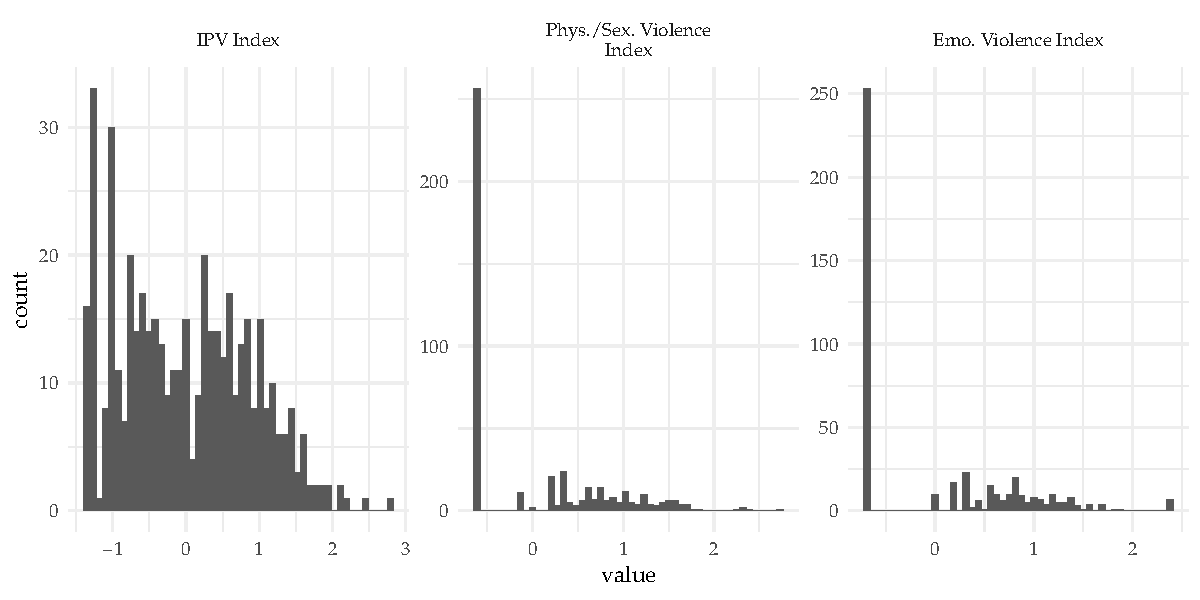
\includegraphics[width = \textwidth]{figures/distribution_violence.pdf}
\caption{Histograms showing distribution of violence outcomes.}
\label{fig:dist_violence}
\end{figure}

\begin{figure}[H]
\centering
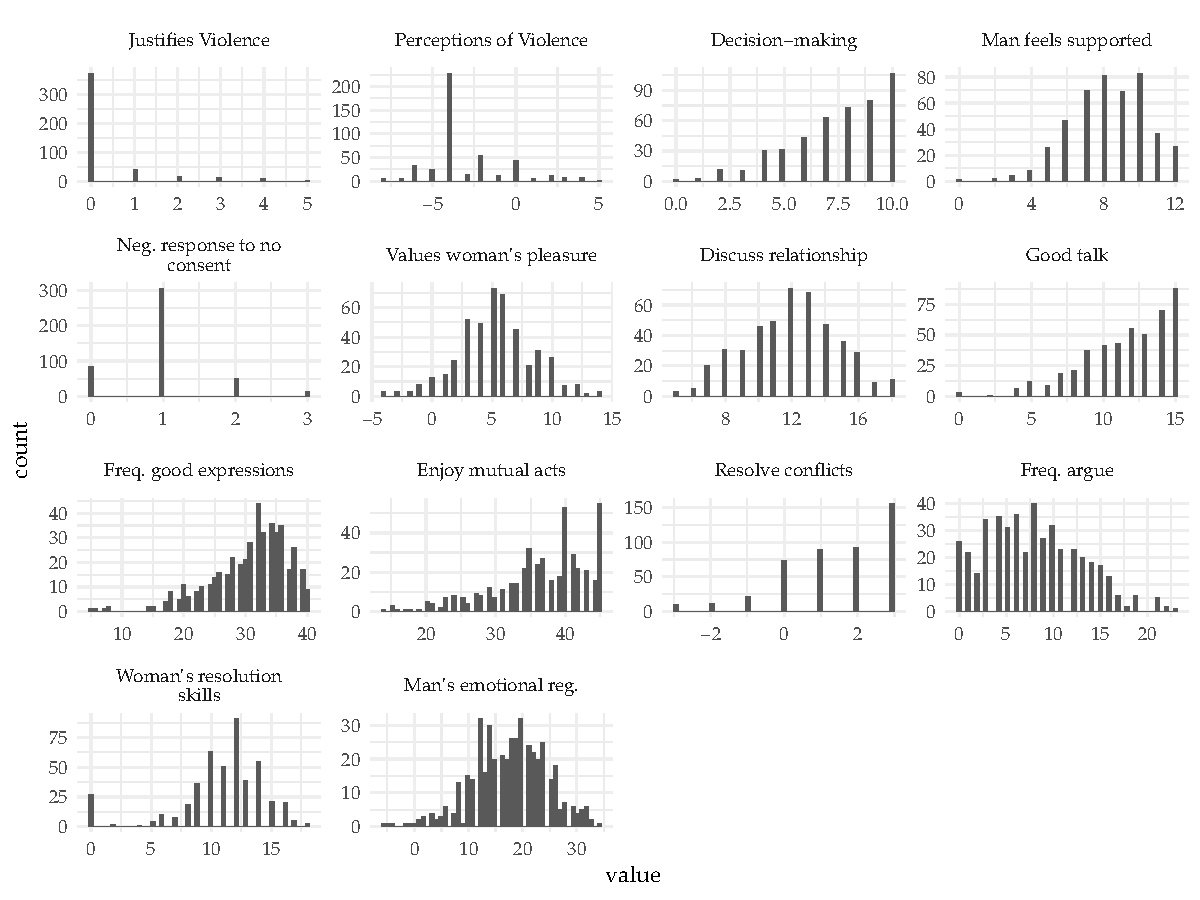
\includegraphics[width = \textwidth]{figures/distribution_mens.pdf}
\caption{Histograms showing distribution of men's outcomes.}
\label{fig:dist_mens}
\end{figure}

\begin{figure}[H]
\centering
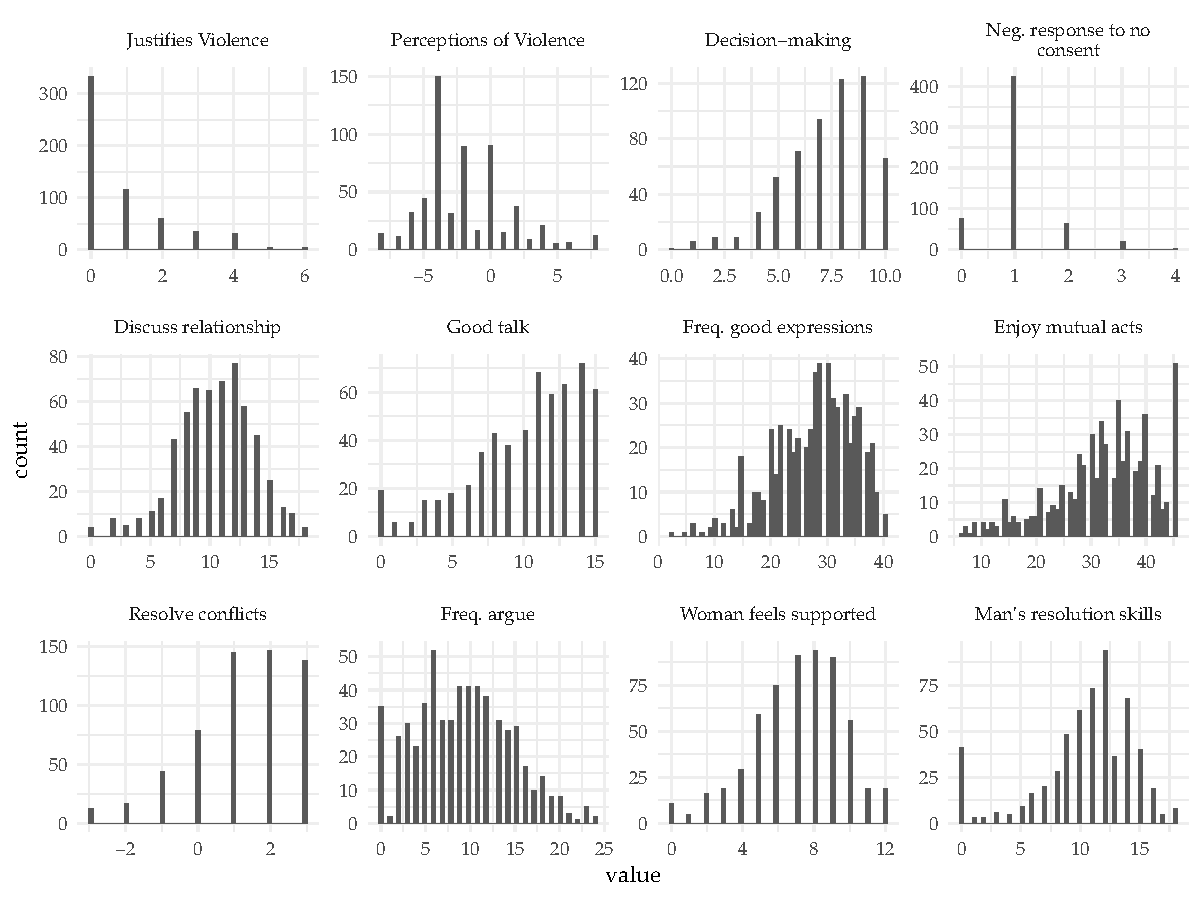
\includegraphics[width = \textwidth]{figures/distribution_womens.pdf}
\caption{Histograms showing distribution of women's outcomes.}
\label{fig:dist_womens}
\end{figure}

\subsection{Covariate balance}

\subsubsection{}

% \begin{table}[H]
% \centering
\begin{table}[H]
\centering
\begin{tabular}{lcccc}
\toprule
\multicolumn{1}{c}{ } & \multicolumn{1}{c}{(1)} & \multicolumn{1}{c}{(2)} & \multicolumn{1}{c}{Diff} & \multicolumn{1}{c}{ } \\
Covariate & MMC & Control & (1) - (2) & $p$-value\\
\midrule
\texttt{age\_m} & 32.15 & 31.34 & -0.80 & 0.41\\
\texttt{childhoodabuse\_index\_m} & 4.64 & 4.45 & -0.19 & 0.55\\
\texttt{emo\_prechr2018\_2pl\_index\_w} & 0.07 & 0.03 & -0.05 & 0.65\\
\texttt{engaged\_m} & 0.16 & 0.16 & 0.00 & 0.92\\
\texttt{girlfriend\_m} & 0.57 & 0.56 & -0.01 & 0.82\\
\addlinespace
\texttt{hscl\_index\_m} & 9.28 & 9.05 & -0.23 & 0.65\\
\texttt{hscl\_index\_w} & 7.78 & 8.28 & 0.50 & 0.26\\
\texttt{literacy\_score\_m} & 4.09 & 3.82 & -0.27 & 0.19\\
\texttt{married\_m} & 0.25 & 0.26 & 0.01 & 0.82\\
\texttt{married\_multiple\_m} & 0.01 & 0.01 & 0.00 & 0.62\\
\addlinespace
\texttt{phys\_sex\_prechr2018\_2pl\_index\_w} & -0.01 & 0.00 & 0.00 & 0.98\\
\texttt{relationship\_years\_w} & 7.08 & 6.44 & -0.64 & 0.16\\
\bottomrule
\end{tabular}
\end{table}

% \caption{Balance of MMC and control clusters on pre-treatment and time invariant coviarates.}
% \label{tab:balance_results}
% \end{table}

\subsubsection{Joint tests}


\subsection{Attrition}

\subsection{Inference}

\begin{table}[H]
\centering
\begin{table}[H]
\centering
\begin{threeparttable}
\begin{tabular}{lccc}
\toprule
\multicolumn{1}{c}{ } & \multicolumn{1}{c}{(1)} & \multicolumn{1}{c}{(2)} & \multicolumn{1}{c}{(3)} \\
Estimator & IPV & Physical/Sexual & Emotional\\
\midrule
CR0 & 0.078 & 0.130 & 0.054\\
 & [0.070] & [0.395] & [0.042]\\
\addlinespace
CR1 & 0.079 & 0.133 & 0.055\\
 & [0.075] & [0.405] & [0.044]\\
\addlinespace
CR2 & 0.085 & 0.141 & 0.059\\
 & [0.095] & [0.433] & [0.063]\\
\addlinespace
CR3 & 0.096 & 0.231 & 0.068\\
 & [0.140] & [0.632] & [0.105]\\
\addlinespace
wild-cluster bootstrap-se (Rademacher) & 0.075 & 0.124 & 0.052\\
 & [0.059] & [0.375] & [0.035]\\
\addlinespace
wild-cluster bootstrap-se (Mammen) & 0.077 & 0.126 & 0.053\\
 & [0.064] & [0.381] & [0.037]\\
\addlinespace
wild-cluster bootstrap-se (Norm) & 0.075 & 0.125 & 0.053\\
 & [0.061] & [0.378] & [0.037]\\
\addlinespace
wild-cluster bootstrap-se (Webb) & 0.076 & 0.125 & 0.052\\
 & [0.064] & [0.377] & [0.036]\\
\addlinespace
cluster pairs bootstrap-se & 0.083 & 0.281 & 0.066\\
 & [0.090] & [0.694] & [0.095]\\
\addlinespace
wild-cluster bootstrap-$t$ (Rademacher) & - & - & -\\
 & [0.119] & [0.414] & [0.088]\\
\addlinespace
wild-cluster bootstrap-$t$ (Mammen) & - & - & -\\
 & [0.129] & [0.459] & [0.085]\\
\addlinespace
wild-cluster bootstrap-$t$ (Norm) & - & - & -\\
 & [0.121] & [0.438] & [0.084]\\
\addlinespace
wild-cluster bootstrap-$t$ (Webb) & - & - & -\\
 & [0.121] & [0.410] & [0.089]\\
\addlinespace
cluster pairs bootstrap-$t$ & - & - & -\\
 & [0.516] & [0.625] & [0.495]\\
\addlinespace
randomization inference $\beta$ & - & - & -\\
 & [0.106] & [0.489] & [0.104]\\
\bottomrule
\end{tabular}
\begin{tablenotes}
\item \textit{Note: } 
\item Comparison of inference from sampling and randomization-based
       uncertainty estimates for pre-registered primary outcomes. Estimated standard errors
       are shown with $p$-value from two-sided hypothesis of no effect shown in parentheses.
       CR0 - CR3 are cluster and heteroskedasticity robust variance estimators as defined in
       The wild cluster bootstrap estimates use the algorithm from Cameron, Gelbach, and Miller (2008)
       with multipliers drawn from either the Rademacher, Mammen, Normal, or Webb distributions.
\end{tablenotes}
\end{threeparttable}
\end{table}

\caption{Comparison of variance estimators for inference for ITT effects.}
\label{tab:inference}
\end{table}

\subsection{Pooled analysis}

\begin{table}[H]
\centering

\begin{tabular}{l c c c c c c}
\toprule
 & IPV & IPV & Physical/Sexual & Physical/Sexual & Emotional & Emotional \\
\midrule
MMC                 & $0.173$        & $0.151$       & $0.122$        & $0.122$       & $0.093$        & $0.057$       \\
                    & $(0.080)$      & $(0.121)$     & $(0.101)$      & $(0.101)$     & $(0.074)$      & $(0.092)$     \\
Constant            & $-0.083$       & $-0.095$      & $-0.092$       & $-0.092$      & $-0.055$       & $-0.043$      \\
                    & $(0.050)$      & $(0.057)$     & $(0.060)$      & $(0.060)$     & $(0.059)$      & $(0.059)$     \\
\midrule
Bootstrap $p$-value & $0.083$        & $0.230$       & $0.243$        & $0.249$       & $0.293$        & $0.548$       \\
Covariates          & $\textrm{Yes}$ & $\textrm{No}$ & $\textrm{Yes}$ & $\textrm{No}$ & $\textrm{Yes}$ & $\textrm{No}$ \\
Clusters            & $16$           & $16$          & $16$           & $16$          & $16$           & $16$          \\
Observations        & $16$           & $16$          & $16$           & $16$          & $16$           & $16$          \\
Adj. R$^2$          & $0.537$        & $0.036$       & $0.029$        & $0.029$       & $0.527$        & $-0.043$      \\
\bottomrule
\multicolumn{7}{l}{\scriptsize{\parbox{\linewidth}{\vspace{2pt} 
       \textit{Notes:} Estimates of the intent-to-treat effects of Modern Man mobile 
       messaging program on pre-registered primary outcomes with data pooled at the block 
       level and using adjusted regression specification based on the Lin 2013 estimator with 
       CR2 cluster-robust standard errors in parentheses. Columns 1 and 2 are a composite 
       index of acts of intimate partner violence. Columns 3 and 4 are a composite index of acts
       of physical violence. Columns 5 and 6 are a composite index of acts of sexual violence.
       All indices were constructed using the first factor from IRT models of subitems. 
       Bootstrap $p$-value estimated using 10,000 replicates of wild cluster bootstrap-$t$. \\ $^{***}p<0.001$; $^{**}p<0.01$; $^{*}p<0.05$.}}}
\end{tabular}

\caption{Pooled ITT effects on indices of intimate partner violence since Christmas 2018 at the cluster level.}
\label{tab:ipv_pooled}
\end{table}

\begin{figure}[H]
\centering
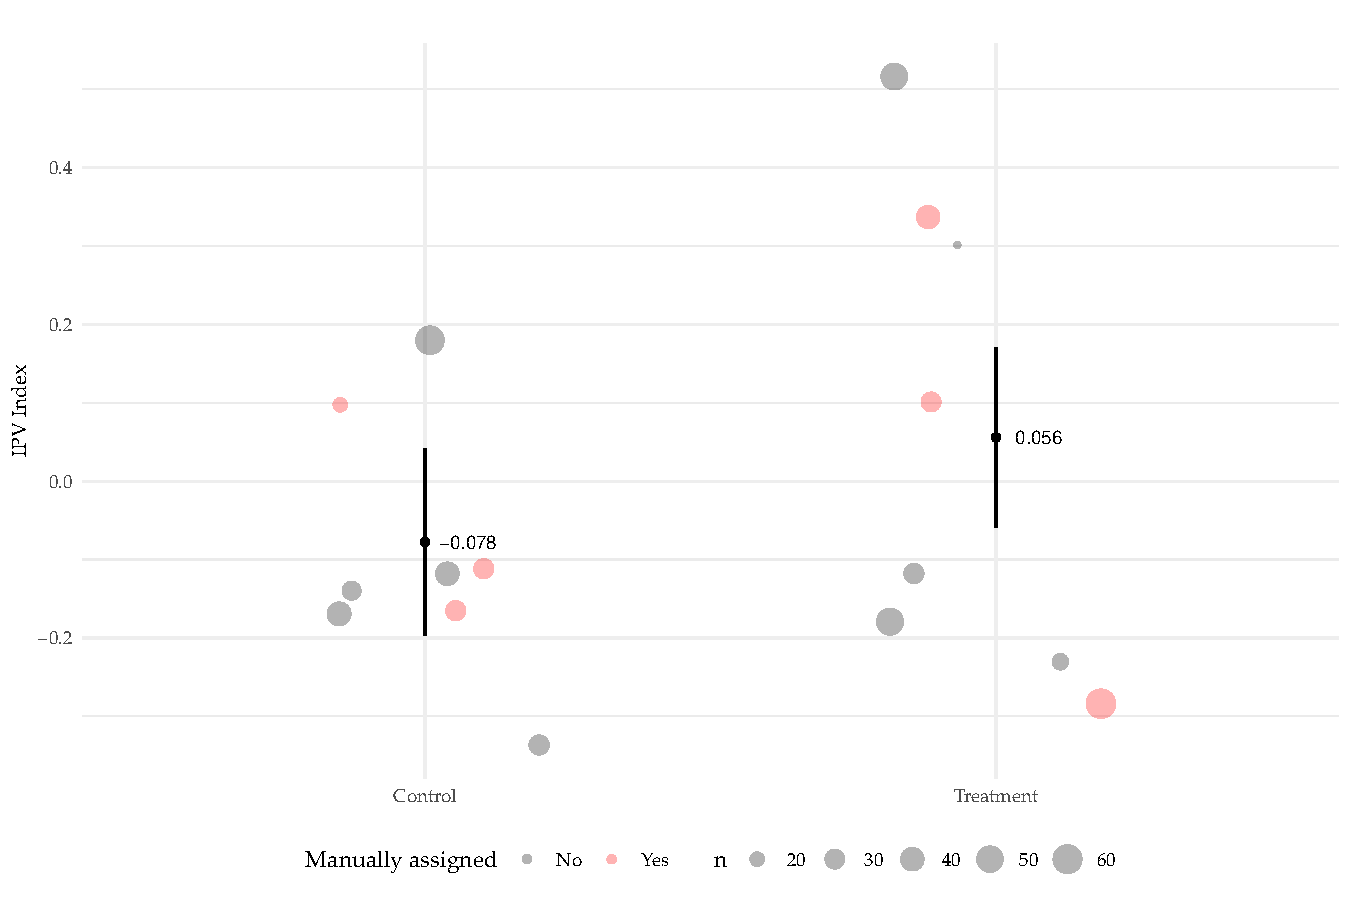
\includegraphics[width = \textwidth]{figures/ipv_pooled.pdf}
\caption{Plot of pooled ITT effects.}
\label{fig:ipv_pooled}
\end{figure}

\subsection{Block assignment}

\begin{table}[H]
\centering

\begin{tabular}{l c c c c c c}
\toprule
 & IPV & IPV & Physical/Sexual & Physical/Sexual & Emotional & Emotional \\
\midrule
MMC                 & $0.142$        & $0.160$        & $0.111$        & $0.112$        & $0.110$        & $0.157$        \\
                    & $(0.085)$      & $(0.154)$      & $(0.141)$      & $(0.403)$      & $(0.059)$      & $(0.097)$      \\
Constant            & $-0.083$       & $-0.109$       & $-0.086$       & $-0.083$       & $-0.037$       & $-0.063$       \\
                    & $(0.064)$      & $(0.085)$      & $(0.063)$      & $(0.072)$      & $(0.054)$      & $(0.081)$      \\
\midrule
Bootstrap $p$-value & $0.118$        & $0.396$        & $0.417$        & $0.816$        & $0.083$        & $0.116$        \\
Covariates          & $\textrm{Yes}$ & $\textrm{Yes}$ & $\textrm{Yes}$ & $\textrm{Yes}$ & $\textrm{Yes}$ & $\textrm{Yes}$ \\
Clusters            & $16$           & $10$           & $16$           & $10$           & $16$           & $10$           \\
Observations        & $455$          & $288$          & $455$          & $288$          & $455$          & $288$          \\
Adj. R$^2$          & $0.422$        & $0.394$        & $0.386$        & $0.333$        & $0.416$        & $0.443$        \\
\bottomrule
\multicolumn{7}{l}{\scriptsize{\parbox{\linewidth}{\vspace{2pt} 
       \textit{Notes:} Estimates of the intent-to-treat effects of Modern Man mobile 
       messaging program on pre-registered primary outcomes using adjusted regression 
       specification based on the Lin 2013 estimator with CR2 cluster robust 
       standard errors in parentheses. Columns 1 and 2 are a composite index of 
       acts of intimate partner violence. Columns 3 and 4 are a composite index of acts
       of physical violence. Columns 5 and 6 are a composite index of acts of sexual violence.
       All indices were constructed using the first factor from IRT models of subitems. 
       Bootstrap $p$-value estimated using 10,000 replicates of wild cluster bootstrap-$t$. \\ $^{***}p<0.001$; $^{**}p<0.01$; $^{*}p<0.05$.}}}
\end{tabular}

\caption{Comparison of results by whether block was min-max randomized only.}
\label{tab:block_rand}
\end{table}

\begin{table}[H]
\centering

\begin{tabular}{l c c c}
\toprule
 & IPV & Physical/Sexual & Emotional \\
\midrule
MMC                             & $0.182$        & $-0.081$       & $0.297$        \\
                                & $(0.303)$      & $(0.288)$      & $(0.178)$      \\
Min-max randomized              & $0.056$        & $-0.067$       & $0.081$        \\
                                & $(0.139)$      & $(0.109)$      & $(0.087)$      \\
MMC $\times$ Min-max randomized & $-0.034$       & $0.128$        & $-0.138$       \\
                                & $(0.179)$      & $(0.150)$      & $(0.107)$      \\
Constant                        & $-0.154$       & $0.001$        & $-0.141$       \\
                                & $(0.210)$      & $(0.171)$      & $(0.156)$      \\
\midrule
Covariates                      & $\textrm{Yes}$ & $\textrm{Yes}$ & $\textrm{Yes}$ \\
Clusters                        & $16$           & $16$           & $16$           \\
Observations                    & $455$          & $455$          & $455$          \\
Adj. R$^2$                      & $0.420$        & $0.384$        & $0.415$        \\
\bottomrule
\multicolumn{4}{l}{\scriptsize{\parbox{\linewidth}{\vspace{2pt} 
       \textit{Notes:} Estimates of treatment effect heterogeneity for the Modern Man mobile 
       messaging program based on randomization type. Estimates are from adjusted regression 
       specification based on the Lin 2013 estimator with CR2 cluster-robust 
       standard errors in parentheses. Column 1 is a composite index of 
       acts of intimate partner violence. Column 2 is a composite index of acts
       of physical violence. Column 3 is a composite index of acts of sexual violence.
       All indices were constructed using the first factor from IRT models of subitems. 
      \\ $^{***}p<0.001$; $^{**}p<0.01$; $^{*}p<0.05$.}}}
\end{tabular}

\caption{ITT treatment effect heterogeneity by whether block was min-max randomized only.}
\label{tab:block_rand_X}
\end{table}


\subsection{Missing data models}

\subsection{Bayes}


%Comments on Table \ref{tab:ipv}
%\begin{itemize}
%  \singlespacing
%  \item All effects are in hypothesized direction. 
%  \item The 
%  \item We s
%\end{itemize}



\end{document}
